\documentclass{article}
\usepackage{amsmath, amssymb, amsthm}
\usepackage{xcolor}
\usepackage{tikz,ifthen}
\usetikzlibrary {arrows.meta,calc,positioning}

\begin{document}

		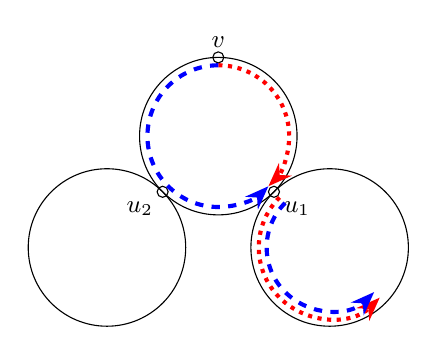
\begin{tikzpicture}
			\draw (0,0) circle[draw=black, radius=1];
			\draw (0.707, -0.707) circle[radius=2pt] node [below right, font=\small] {$ u_1 $};
			\draw (-0.707, -0.707) circle[radius=2pt] node [below left, font=\small] {$ u_2 $};
			\draw (0, 1) circle[radius=2pt] node [above, font=\small] {$ v $};
			\draw (1.414,-1.414) circle[draw=black, radius=1];
			\draw (-1.414,-1.414) circle[draw=black, radius=1];

                \draw[-{Stealth[length=3mm]},color=red,dotted, line width=1.5pt] (0,0.9) arc (90:-45:.9);
                \draw[-{Stealth[length=3mm]},color=red,dotted, line width=1.5pt] (0.7777,-0.7777) arc (135:315:.9);

                \draw[-{Stealth[length=3mm]},color=blue, dashed, line width=1.5pt] (0,0.9) arc (90:315:.9);
                \draw[-{Stealth[length=3mm]},color=blue, dashed, line width=1.5pt] (0.8484,-0.8484) arc (135:315:.8);
		\end{tikzpicture}

\end{document}